\chapter{Interview questions}\label{Interview:questions} 

\begin{itemize}
 \item Do you find that student appreciate e-tools?
 \begin{itemize}
 \item Which tools do you think is needed to engage students?
 \end{itemize}
 
 \item A large problem (at least at the computer science program) is that may students are shy and doesn't dare to ask questions. Do you think that an e-tool in the classroom could simply this. e.g. anonymous feedback services? 

 
 \item Do you experience that there is different types of students that response on different types of motivation?
 \begin{itemize}
 \item If so, which trends have you experienced?
 \item Do you think that it is possible to reach more students by e-tools?
 \end{itemize}
 
 \item Are you familiar with gamification?
 \begin{itemize}
 \item How did you get it?
 \item Which pro and cons do you see?
 \item Which pitfalls have you experienced?
 \end{itemize}
 
 \item  How much time would you as a teacher be able to spend to create assignments?
 \begin{itemize}
 \item How much time do you spent on creating regular assignments?
 \end{itemize}
 
 \item What do you need available to see that this tool will work?
 \begin{itemize}
 \item Which difficulties do you see by using a e-tool, e.g. Tech.io?
 \end{itemize}
\item How can we motivate you as a teacher?
\item What would you think about if you should create a similar tool?

\end{itemize}
\chapter{Workshop scenarios}\label{Worskshop:senarios}
\textbf{Introduction 10min}
We are studying the fifth year at computer science program at LTU and for now doing our project. As a part of our prestudy are we hosting this workshop where we will investigate possibilities through a couple of scenarios. You will do a couple of assignments in groups and then present your result and discuss these with others.\\

\textbf{Scenario 1 10 min + 10 min discussion}\\
You have just started a course where you will learn to program in a language you don't find interesting. The teacher has given you lot recommended assignments but non seems interesting. Which type of system or moments would motivate you to do the assignments. Dream free.
\begin{itemize}
\item Which subject do you think has this problem?
\item Do the assignment needs to be presented? If so how?
\item Which material is needed?
\item What should be on a list with highlights?
\end{itemize} 

\textbf{Scenario 2 10 min + 10 min discussion}
After many years you are the teacher for that boring course. The boss comes in to your office a Friday afternoon and says that the course moments are to few and you need to update them till Monday. You sits down as the motivated teacher you are and thinks about a system than would motivate students, you remember your old concept. \\
You want to make this work for a long time, which limitations must you as a teacher do?\\
\begin{itemize}
\item What is most time consuming?
\item Is it possible to sort your highlight after time consuming?
\item How long time can the moment take to develop and maintain?
\end{itemize} 

\textbf{Scenario 3 15 min + 10 min discussion}
Now when you have a working system and it scales along the new courses you teach in, but the students wants a e-tool. How does this tool look like?, Think web besides details and try to catch the users experience.

\begin{itemize}
\item How do you do inputs?
\item How does your highlights look like practical?
\item Do you see any limitations?
\end{itemize} 

\chapter{Installation instructions}
Learning as a service was built and tested on debian linux 9 (stretch) with node 8.6.0 and npm 5.3.0.
\section{Tester}
Tester consists of two components; Manager and Runner. Managaer replies to requests from the backend and manages docker containers that run arbitrary code. Containers are used to ensure that some test A does not interfere with some later test B by modifying the executing environment.\\
\begin{enumerate}
    \item Clone the repo: \textbf{git clone https://github.com/ax-rwnd/d7017e-project}
    \item Change directory to the Manager folder: \textbf{cd d7017e-project/tester}
    \item Install the dependencies for the Manager: \textbf{npm i}
    \item (Optional) Select languages by adding/removing dependencies in \textbf{Makefile}. For instance the line\textbf{ all: python27 python3 java c \# haskell} selects the languages Python 2.7, Python 3, Java, C, but not Haskell (since it's commented out).
    \item Run the Makefile: \textbf{make}
    \item (Optional) Set preferences for Runner in \textbf{config/default.js}. There, things like queue lengths and ports may be configured.
    \item Move back up to manager: \textbf{cd ..}
    \item Start Manager: \textbf{node server.js \{PORT\}}
\end{enumerate}

\section{Backend}
Backend is the state-managing component. It uses MongoDB to store information that it receives while processesing frontend requests and tester results.
\begin{enumerate}
\item Install och configure MongoDB.
\item Clone the repo: \textbf{git clone https://github.com/ax-rwnd/d7017e-project}
\item Change directory to backend: \textbf{cd d7017e-project/Backend}
\item Install dependencies: \textbf{npm i}
\item onfigure database address/port in \textbf{Backend/config/default} and \textbf{Backend/config/production}. IP/Port may differ between the files, should you want to use different databases for testing and production. To select one of these files, set the \textbf{NODE\_ENV} environment variable to \textbf{production} or \textbf{development}.
\item Start the backend daemon: \textbf{npm start}.
\item (Optional) Start start backend in the foreground: \textbf{node ./bin/www}
\end{enumerate}

\section{Frontend}
Frontend is the part that the users see. It builds on Angular for UI and contacts backend for functionality.

\begin{enumerate}
    \item Clone the repo: \textbf{git clone https://github.com/ax-rwnd/d7017e-project}
    \item Change directory to frontend: \textbf{cd d7017e-project/frontend}
    \item Redirect frontend to backend: \textbf{sed -i "s/ \textbackslash (backend\_ip: \textbackslash )'.*'/ \\ \textbackslash 1'https://{your\_backend}'/" src/environments/environment.prod.ts}
    \item Tell were the global ip for frontend is: \textbf{ed -i "s/\textbackslash (frontend\_ip: \\ \textbackslash)'.*'/\textbackslash 1'https://{your\_frontend}'/" src/environments/environment.prod.ts}
    \item (Optional) Repeat step 2 and 3 for \textbf{src/environments/environment.ts}
    \item Move or link your ssl-certificates \textbf{ln -s encryption/private.key.default encryption/private.key \&\& ln -s encryption/server.crt.default encryption/server.crt}
    \item Start server: \textbf{--ssl 1 --ssl-cert ./encryption/server.crt --ssl-key ./encryption/private.key --live-reload false}
\end{enumerate}

\chapter{Cas-diagram}
\begin{figure}[H]
\centering
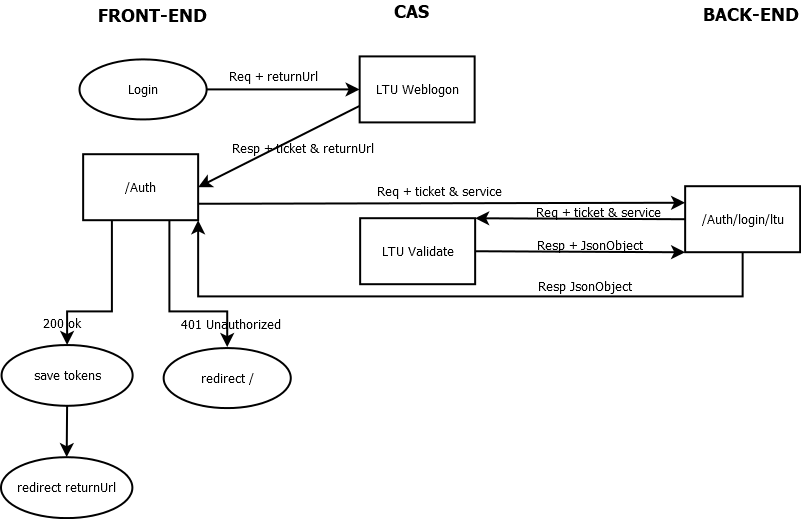
\includegraphics[scale=0.45]{img/login.png}
\caption{A diagram showing how CAS-login is implemented.}
\end{figure}
